
\chapter{Computing Performance \label{chpt:seq-code-performance}}

This section evaluates the computing performance (timing) of the code.
Our goal is to show that the new algorithm of angular convolution
is much faster than the old naive one; the huge amount of simulation
during this thesis has proven that it is indeed the case. The purpose
of this section is to substantiate that statement by a proper and
systematic performance evaluation.

Firstly, we will evaluate the performance only concerning
the $\mathcal{F}_{\mathrm{exc}}$ term, knowing that the two other
terms of the functional, the $\mathcal{F}_{\mathrm{id}}$ and $\mathcal{F}_{\mathrm{ext}}$
contribution, require a computer time of the same magnitude as the
new algorithms for $\mathcal{F}_{\mathrm{exc}}$ part. The spatial
and angular grid dependence of the various branches are discussed.

\section{FFT}

The \acs{FFT}, which is used by the spatial convolution and the \acs{FGSHT}
process, play an important role in the implementation. 

\begin{figure}[H]
\begin{centering}
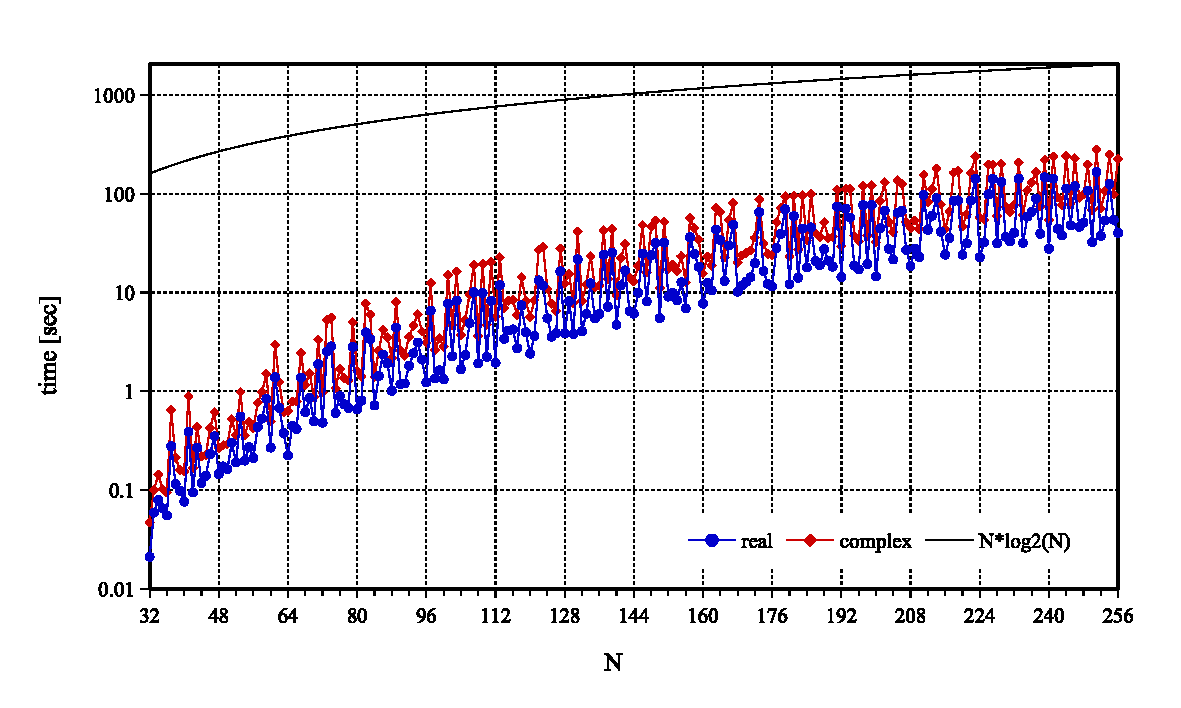
\includegraphics[bb=0bp 20bp 567bp 310bp,width=1\columnwidth]{_figure/results/fftw_timing}
\par\end{centering}
\caption{Timing of \acs{FFT} for real-to-complex and complex-to-complex processes
with respect to grid number $N$\label{fig:timing-FFT}}
\end{figure}

Referring to figure \ref{fig:timing-FFT}, the expected dependance
on $O(N\log_{2}N)$ \citep{Numerical_Recipes_3ed} does not totally
exist, but it appears to be of the same form, depending on the algorithm
of \acs{FFT} \citep{Briggs-DFT}. It should be noted that a grid
of prime number is always at the peak in each figure, which means
it can be twice as long or more than that of a nearby composite number.
Therefore it is better to use an even number grid, for which the $k$-border
correction in $\mathsection$\ref{subsec:k-border-effect} should
absolutely be accounted for. Apart from this, to compare
the algorithms for angular integration involved in this thesis, we
are not really interested in computing performance with respect to
the number of spatial grid. However, the ratio of real and complex
\acs{FFT} timing is important, as illustrated in figure \ref{fig:fft-real-to-complex},
where the ratio between real-to-complex and complex-to-complex \acs{FFT}
processes is measured as 0.54, near the theoretical ratio 0.5. For
example, we may process $n_{\mathrm{angle}}$ real to complex \acs{FFT},
then $n_{\mathrm{spatial}}/2$ complex to complex \acs{FGSHT}. Or
we may process $n_{\mathrm{spatial}}$ real to complex \acs{FGSHT},
then $n_{\mathrm{proj}}/2$ complex to complex \acs{FFT}. This should
not give a significant difference if $n_{\mathrm{angle}}\sim n_{\mathrm{proj}}$
for small $n_{\max}$. If the ratio is not 1:2, it will have an influence
on the choice of algorithm.
\begin{center}
\begin{figure}[h]
\begin{centering}
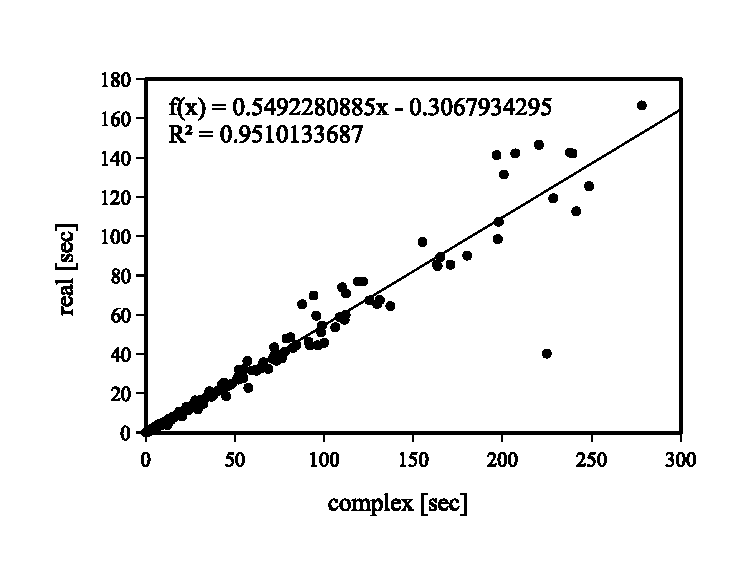
\includegraphics[bb=0bp 20bp 340bp 235bp,width=0.55\columnwidth]{_figure/results/fftw_real_v_cmplx}
\par\end{centering}
\caption{Timing of real-to-complex \acs{FFT} processes with respect to its
complex-to-complex process of the same grid number $N$\label{fig:fft-real-to-complex}}
\end{figure}
\par\end{center}

\section{FGSHT}

The computing times of \acs{GSHT} and \acs{FGSHT} are shown in figure
\ref{fig:time-gsht-fgsht}. There is no reason to view in detail how
much \acs{FFT} has accelerated the \acs{GSHT} process, but clearly
\acs{FGSHT} can be 100 times faster than \acs{GSHT}. In addition, looking
at the influence of the symmetry in $\Psi$ on \acs{GSHT}, $s=1$
is on average 5 times longer than $s=2$ ($s$ being the \acs{MRSO}
defined in $\mathsection$\ref{sec:fgsht}). As accuracy tests show
that \acs{GSHT} and \acs{FGSHT} give exactly the same result, and
as the case $m_{\max}<n_{\max}$ is never needed, it is possible to
utilize \acs{FGSHT} in all the cases to have a faster performance.
\begin{center}
\begin{figure}[H]
\begin{centering}
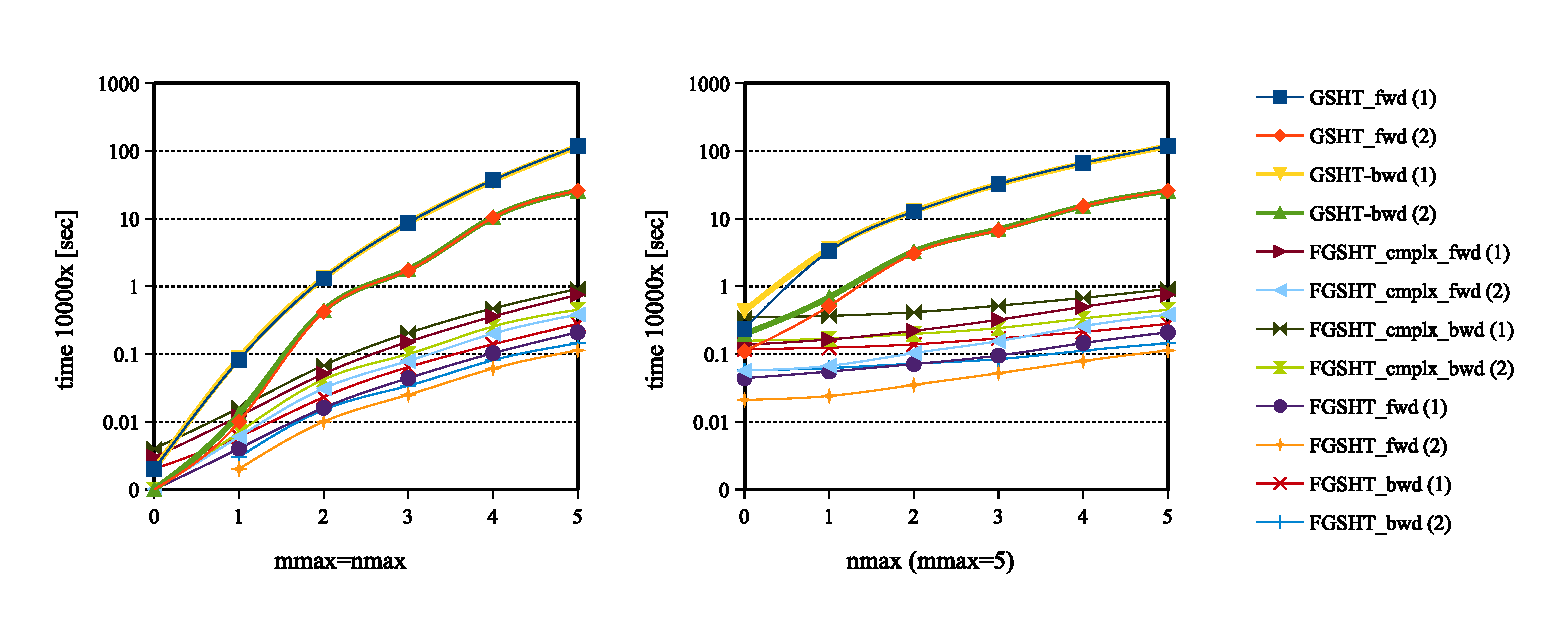
\includegraphics[bb=0bp 20bp 731bp 263bp,width=1\columnwidth]{_figure/results/fgsht_perf}
\par\end{centering}
\caption[Computing time of \acs{GSHT} and \acs{FGSHT}]{Computing time of \acs{GSHT} and \acs{FGSHT} (per 10000 times),
between parentheses is the order of symmetry axes $s$\label{fig:time-gsht-fgsht}}
\end{figure}
\par\end{center}

However, it is important to know the ratio between real and complex
\acs{FGSHT} processes for the same reason as \acs{FFT}. It is demonstrated
that this number is 0.3 in all cases, and it does not depend on $m_{\max}$,
$n_{\max}$ or $s$. The difference between these two is that the
real one performs real-to-complex \acs{FFT} for the $\Phi,\Psi$
grid and calculates only slightly more than half of projections ($\mu\geq0$)
than the complex one.\textcolor{red}{{} }Theoretically, the ratio should
be greater than 0.5. This could mean there may be an extra process
in the complex one, or it is controlled by the memory. Ultimately,
the final result 0.3 means that doing $n_{\mathrm{spatial}}$ real
to complex \acs{FGSHT} should take only 0.6 the time of doing $n_{\mathrm{spatial}}/2$
complex to complex \acs{FGSHT}, which means in \texttt{\textbf{convolution\_standard}}
we should use less time to compute \acs{FGSHT} than in \texttt{\textbf{convolution\_pure\_angular}},
which is in fact not observed in the following tests.
\begin{center}
\begin{figure}[H]
\begin{centering}
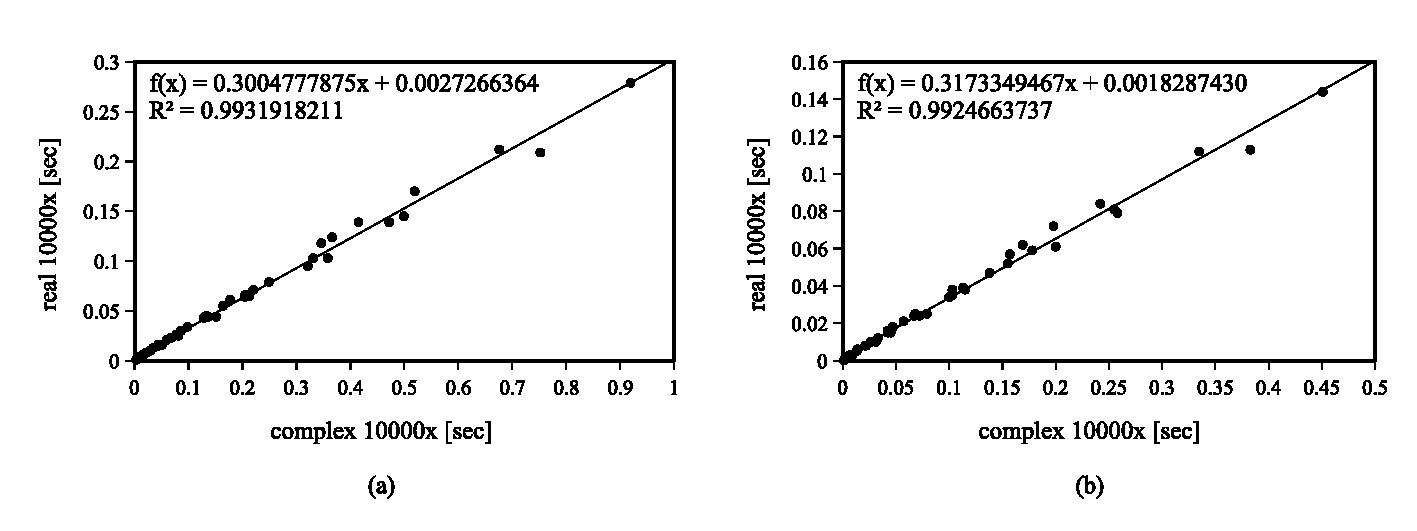
\includegraphics[bb=20bp 20bp 660bp 235bp,width=1\columnwidth]{_figure/results/fgsht_real_v_cmplx}
\par\end{centering}
\caption[Timing of real-to-complex \acs{FGSHT} processes with respect to its
complex-to-complex process of the same $m_{\max}$ and $n_{\max}$]{Timing of real-to-complex \acs{FGSHT} processes with respect to
its complex-to-complex process of the same $m_{\max}$ and $n_{\max}$,
for $s=1$ and $s=2$\label{fig:fgsht-real-to-complex}}
\end{figure}
\par\end{center}

\section{$k$-kernel\label{sec:-kernel}}

As discussed in the previous section, the final result of energy and
structure is independent of the choice of path inside a $k$-kernel.
That means we are free to choose the fastest path. Path (1) passing
directly by $\hat{c}(k,\mathbf{\Omega}_{1},\mathbf{\Omega}_{2})$
in figure \ref{fig:k-kernel} has no interest in timing, as the memory
limit does not support such a direct algorithm for the entire $k$-space.
Here we only compare the paths (2), (3) and (4), which correspond
to eq. (\ref{eq:gamma-k}), (\ref{eq:im}) and (\ref{eq:gamma-blum}).

The theoretical predictions for the computing time of \acs{OZ} equation
with $m_{\max}=n_{\max}$ are listed in table \ref{tab:FE-of-OZ}.
If the \acs{OZ} equation is the most time-consuming part, the observed
result should have the same tendency. Figure \ref{fig:Timing-k-kernel}
shows the experimental timing of the three paths, where path (3) is
100 times longer than (4), corresponding well to the theoretical value.
Path (2) is much longer than path (3) because apart from the \acs{OZ}
equation, the reading in memory and calculation of the \acs{DCF}
mentioned in $\mathsection$\ref{chpt:fft-spatial} also takes time.

\begin{figure}[H]
\begin{centering}
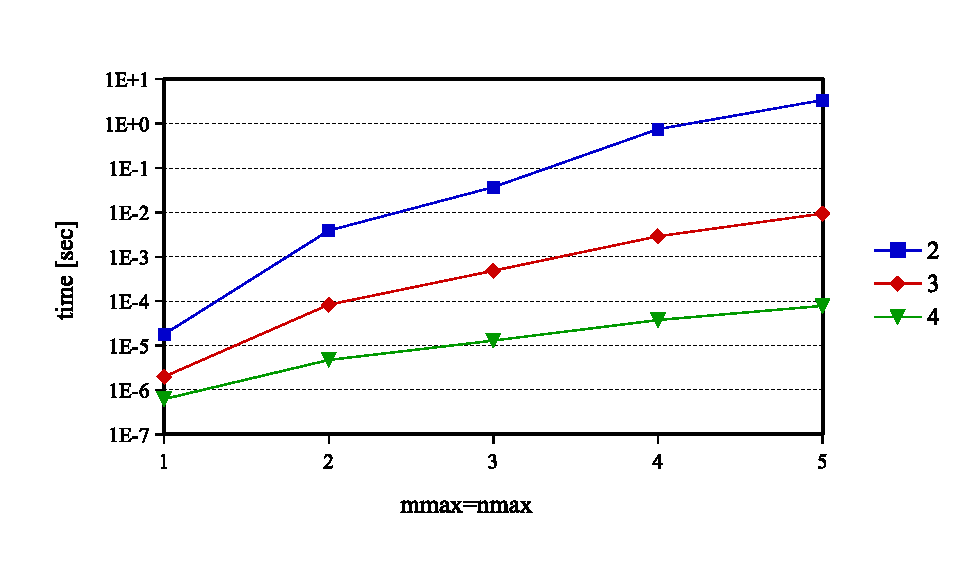
\includegraphics[bb=0bp 20bp 504bp 196bp,width=0.75\columnwidth]{_figure/results/k-kernel}
\par\end{centering}
\caption[Timing of a $k$-kernel]{Timing of a $k$-kernel (log scale)\label{fig:Timing-k-kernel}}
\end{figure}


\section{Entire iteration of $\mathcal{F}_{\mathrm{exc}}$ evaluation}

Apart from all the \texttt{\textbf{naive}} methods that will be discussed
in $\mathsection$\ref{subsec:Comparison-between-naive_standar},
figure \ref{fig:Entire-iteration} shows all the comparable \texttt{\textbf{convolution}}
timing data. We can see that \texttt{\textbf{convolution\_standard}}
is the fastest algorithm, and \acs{OZ} equation is not the longest
part in the iteration. All the tests are performed for a $L=24$,
$\mathrm{nfft}=72$ grid with 4 series: the three \texttt{\textbf{convolution}}
methods with $m_{\max}=n_{\max}$, and \texttt{\textbf{convolution\_standard}}
with $m_{\max}=5$, varying $n_{\max}$.

\begin{figure}[H]
\begin{centering}
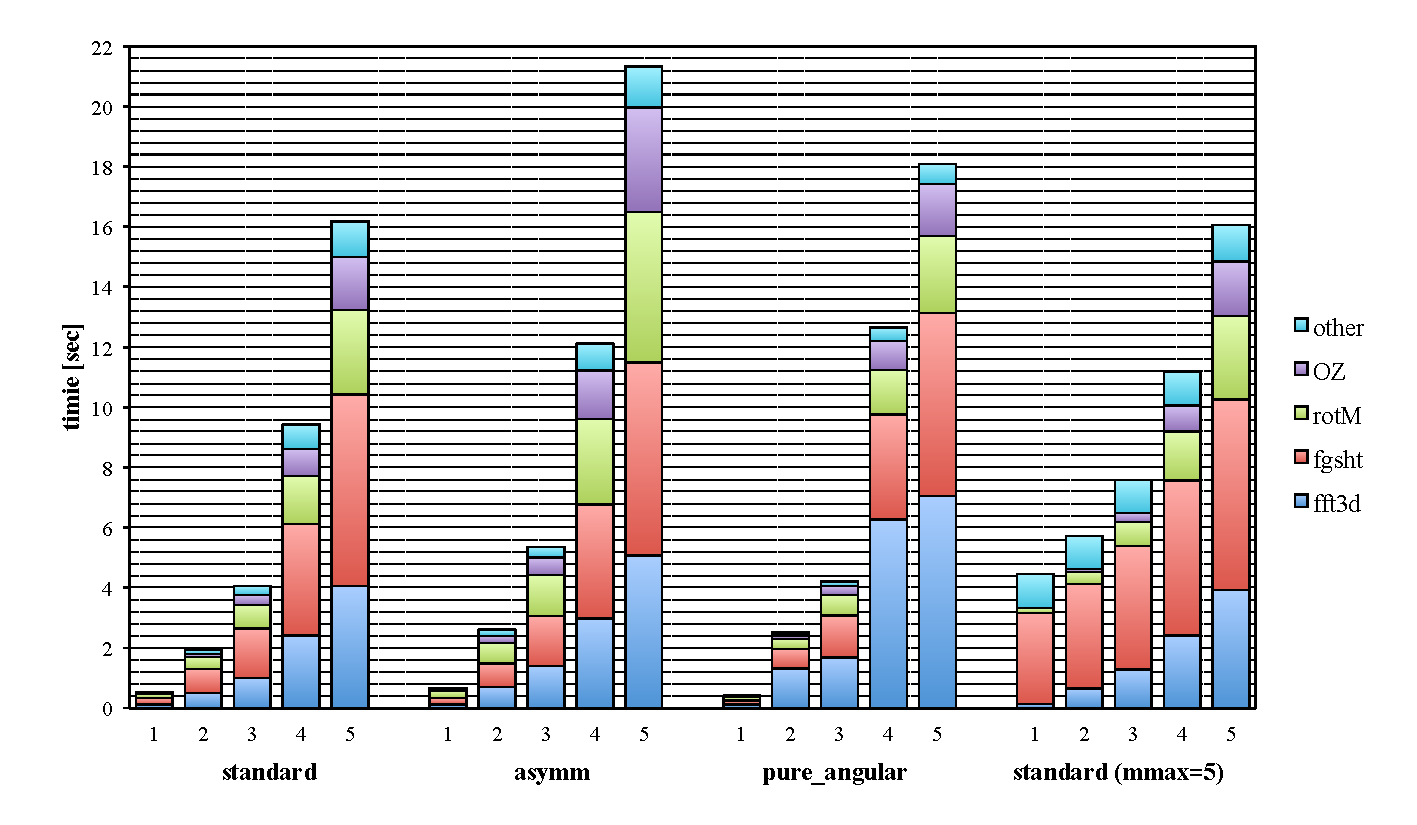
\includegraphics[width=0.9\columnwidth]{_figure/results/branch_perf}
\par\end{centering}
\caption[Entire iteration of $\mathcal{F}_{\mathrm{exc}}$ evaluation]{Entire iteration of $\mathcal{F}_{\mathrm{exc}}$ evaluation: timing
overall / decomposition of timing for 1 iteration evaluation\label{fig:Entire-iteration}}
\end{figure}


\subsection{``naive'' methods and ``convolution\_pure\_angular''\label{subsec:Comparison-between-naive_standar}}

The \texttt{\textbf{naive\_standard}}, \texttt{\textbf{naive\_interpolation}},
and \texttt{\textbf{convolution\_pure\_angular}} methods share the
same processes out of the $k$-kernel. Table \ref{tab:Timing-loop-k}
shows the timing of loop $k$ of these three methods. It indicates
that \texttt{\textbf{convolution\_pure\_angular}} takes far less time
than the other two methods, of which the loop $k$ takes time on the
same order of magnitude as the rest of the iteration. And once $m_{\max}\geq2$,
\texttt{\textbf{naive\_interpolation}} is faster than \texttt{\textbf{naive\_standard}}.
Note that order 2 of \texttt{\textbf{naive\_interpolation}} can give
good results for a \acs{DCF} of $n_{\max}=5$. So in every case of
\texttt{\textbf{naive}} methods, \texttt{\textbf{naive\_interpolation}}
should be used. This verifies the conclusion of $k$-kernel test in
that the path (4) in figure \ref{fig:k-kernel} is the fastest.

\begin{table}[H]
\begin{centering}
\begin{tabular}{ccccc}
\toprule 
$m_{\max}$ & \texttt{\textbf{naive\_standard}} & \texttt{\textbf{naive\_interpolation}} & \texttt{\textbf{convo\_pure\_angular}} & \tableheadline{Other}\tabularnewline
\midrule
1 & 2.34 & 4.42 & 0.26 & 0.15\tabularnewline
2 & 365.95 & 209.12 & 1.09 & 1.43\tabularnewline
3 & 3295.00 & 752.70 & 2.37 & 1.85\tabularnewline
4 & too long & too long & 5.93 & 6.73\tabularnewline
5 & too long & too long & 10.36 & 7.73\tabularnewline
\bottomrule
\end{tabular}
\par\end{centering}
\caption[Timing of loop $k$]{Timing {[}sec{]} of loop $k$ of ``naive\_standard'', ``naive\_interpolation''
and ``convolution\_pure\_angular'', and the rest of iteration\label{tab:Timing-loop-k}}
\end{table}


\subsection{``convolution\_standard'' and ``convolution\_pure\_angular''}

The comparison of \texttt{\textbf{convolution\_standard}} and \texttt{\textbf{convolution\_pure\_angular}}
appears in figure \ref{fig:comparison-pure_angular}. Their difference
lies in the inversion of \acs{FFT} and \acs{FGSHT}. We can see the
other parts are almost identical, but the implementation of \acs{FFT}
is different in terms of time, because in \texttt{\textbf{convolution\_standard}}
the number of \acs{FE} we need for \acs{FFT} is the number of projections,
and in \texttt{\textbf{convolution\_pure\_angular}} it is the number
of angular grid nodes. As there are fewer projections than angular
nodes, \texttt{\textbf{convolution\_standard}} reasonably takes less
time. The stepwise form of the \texttt{\textbf{pure\_angular}} curve
is due to the grid in $\Psi$, which requires $\left\lfloor m_{\max}/2\right\rfloor $
points in the case of $\mathrm{C}_{2v}$ symmetry. Projections are
less sensitive to this effect.

\begin{figure}[H]
\begin{centering}
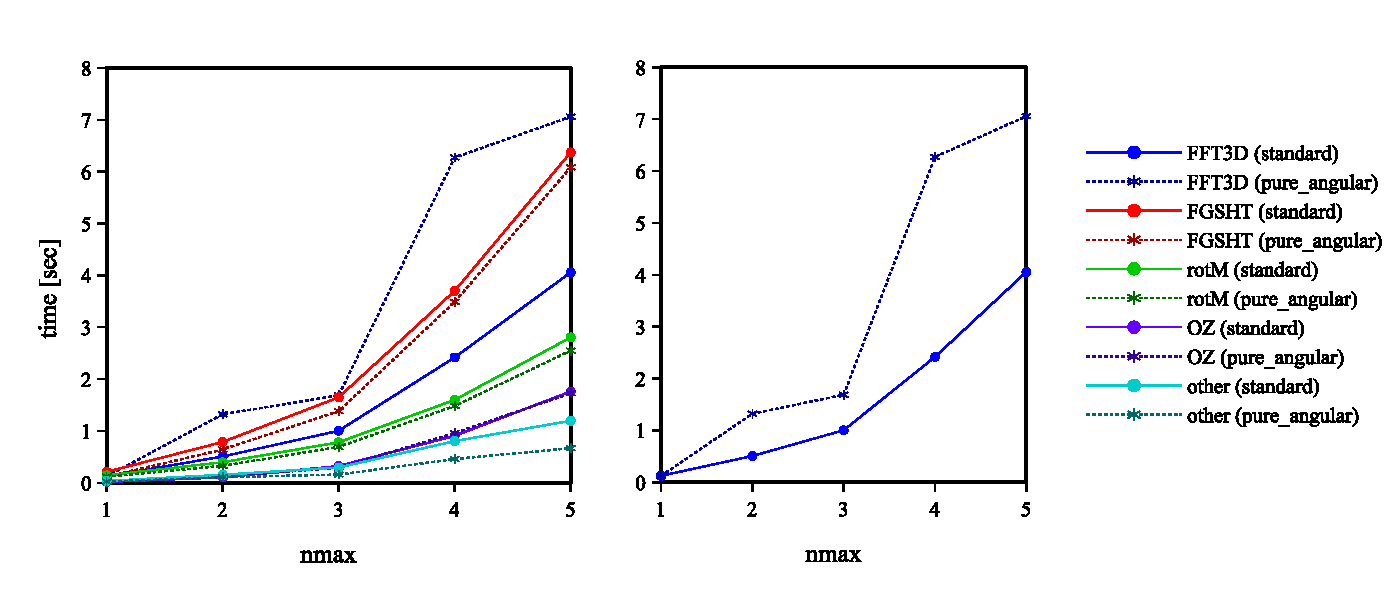
\includegraphics[bb=20bp 20bp 667bp 268bp,width=1\columnwidth]{_figure/results/pure_angular}
\par\end{centering}
\caption[Performance comparison of ``convolution\_standard'' and ``convolution\_pure\_angular'']{Performance \texttt{\textbf{convolution\_standard}} vs \texttt{\textbf{convolution\_pure\_angular\label{fig:comparison-pure_angular}}}}
\end{figure}


\subsection{``convolution\_standard'' and ``convolution\_asymm''}

We compare\texttt{\textbf{ convolution\_standard}} and \texttt{\textbf{convolution\_asymm}}
in figure \ref{fig:comparison-asymm}. The difference is that \texttt{\textbf{standard}}
calculates half of the $k$'s in the $k$-loop and \texttt{\textbf{asymm}}
calculates all $k$'s in the $k$-loop. They share the same process
of \acs{FGSHT}, while for the processes in a $k$-loop (rotM, OZ)
\texttt{\textbf{asymm}} always takes longer. Since in \texttt{\textbf{asymm}}
we calculate the \acs{FFT} for all the projections and in \texttt{\textbf{standard}}
we calculate only a half projections with $\mu\geq0$, the time consumed
by \acs{FFT} is also different.

\begin{figure}[H]
\begin{centering}
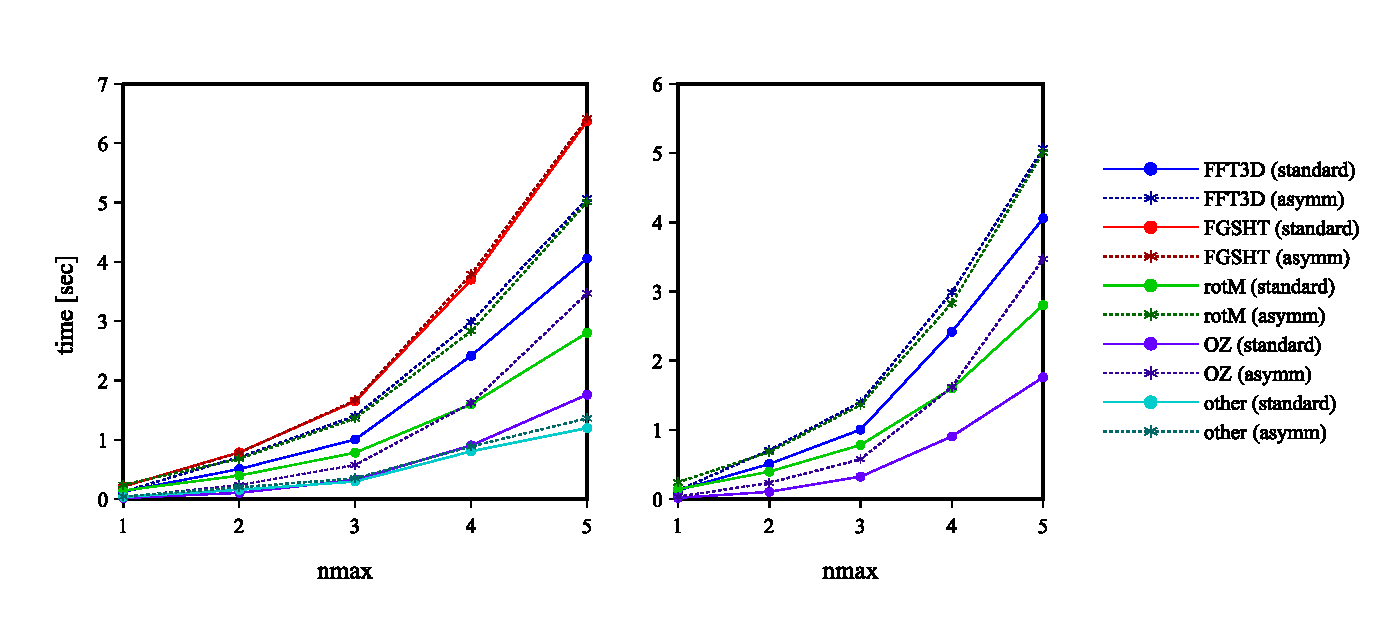
\includegraphics[bb=20bp 20bp 647bp 268bp,width=1\columnwidth]{_figure/results/asymm}
\par\end{centering}
\caption[Performance comparison of ``convolution\_standard'' and ``convolution\_asymm'']{Performance \texttt{\textbf{convolution\_standard}} vs \texttt{\textbf{convolution\_asymm\label{fig:comparison-asymm}}}}
\end{figure}


\subsection{Distinction of $m_{\max}$ and $n_{\max}$}

The comparison of $m_{\max}=n_{\max}$ and $m_{\max}=5$ for\texttt{\textbf{
convolution\_standard}} is shown in figure \ref{fig:comparison-nmax}.
We see that the choice of quadrature order $m_{\max}$ only affects
the \acs{FGSHT} process and the reading/storage of density variable
(other). The time taken by extra order $m_{\max}$ is not cost-free,
so as discussed in the last section, it is fully recommended to use $m_{\max}=n_{\max}$.

\begin{figure}[H]
\begin{centering}
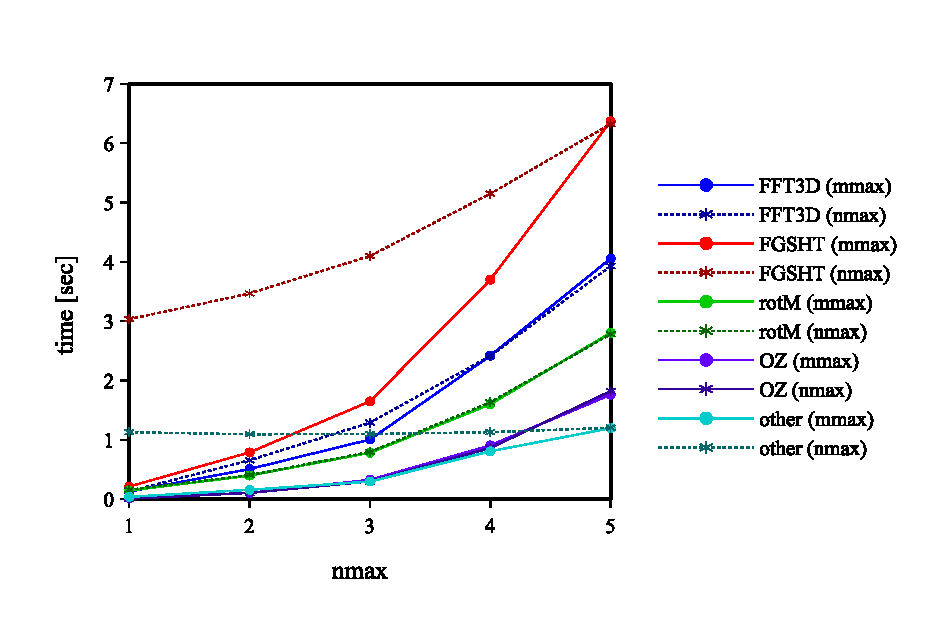
\includegraphics[bb=20bp 20bp 639bp 268bp,width=1\columnwidth]{_figure/results/nmax}
\par\end{centering}
\caption[Performance comparison of ``convolution\_standard'' for $m_{\max}=n_{\max}$
and $m_{\max}=5$]{Performance \texttt{\textbf{convolution\_standard}} for $m_{\max}=n_{\max}$
and $m_{\max}=5$\label{fig:comparison-nmax}}
\end{figure}


\section{Global view of the code performance}

Figure \ref{fig:Timing-full} gives the timing of the whole $\mathcal{F}$
iteration. We can see that the evaluation of $\mathcal{F}_{\mathrm{exc}}$
is at the same order of magnitude as the other two terms and the same
dependency on angular grid. That means that considering the priority
of code optimization, the $\mathcal{F}_{\mathrm{exc}}$ is no longer
an absolute bottleneck to the whole process, owing to the new algorithm.

\begin{figure}[H]
\begin{centering}
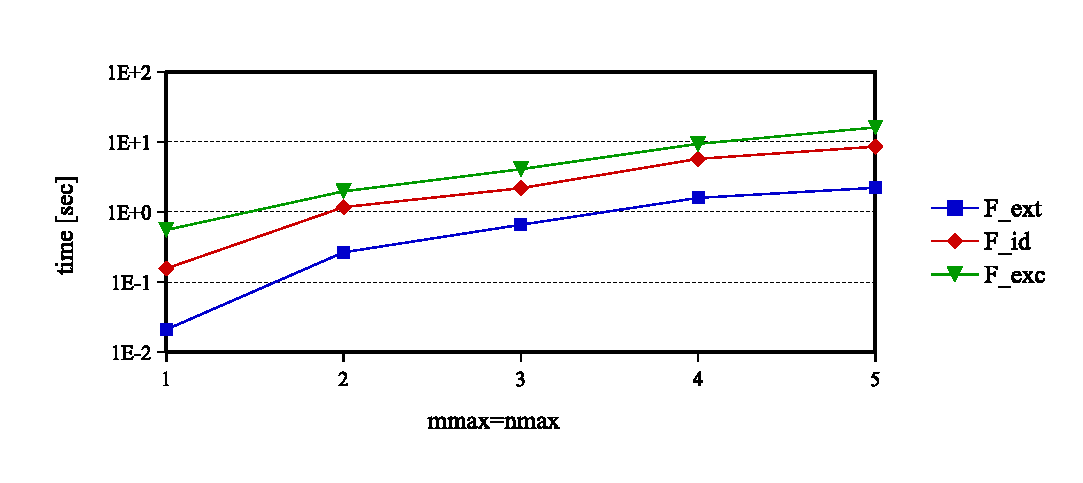
\includegraphics[bb=0bp 20bp 504bp 196bp,scale=0.7]{_figure/results/global_perf}
\par\end{centering}
\caption[Timing of the whole $\mathcal{F}$ iteration]{Timing of the whole $\mathcal{F}$ iteration with $\mathrm{nfft}/L=72/24$
grid (log scale), using \texttt{\textbf{convolution\_standard}} algorithm
\label{fig:Timing-full}}
\end{figure}

In conclusion, we stress that:
\begin{itemize}
\item \texttt{\textbf{convolution\_standard}} is the fastest algorithm among
those that we have tested. The \texttt{\textbf{convolution}} methods
are orders of magnitude faster than \texttt{\textbf{naive}} methods.
It means that we have been able to reduce a complex spatial and angular
convolution process to roughly the same computer cost as a local calculation
in both space and angles, which can be seen as the major accomplishment
of this thesis.
\item The attempt to fix $m_{\max}$ considerably damages the efficiency,
in addition to the necessity; $m_{\max}=n_{\max}$ is absolutely recommended.
\end{itemize}

